\chapter{Estado del Arte y Marco Teórico-Conceptual}\label{chapter:state-of-the-art}

\section{Fundamentos de la Planificación Automática}

La \textit{Planificación Automática} (\textit{Automated Planning}, AP) es una subdisciplina de la inteligencia artificial centrada en la síntesis de secuencias de acciones para alcanzar un objetivo a partir de un estado inicial, sujeto a las restricciones impuestas por el entorno o dominio \parencite{tantakoun2025llms}. Su variante más reconocida es el \textit{problema clásico de planificación} (\textit{Classical Planning Problem}), que se formula bajo un conjunto de supuestos idealizados: el entorno es discreto, determinista, estático, completamente observable y monolítico (de un solo agente) \parencite{peter2021modern}. Este tipo de entorno permite diseñar agentes planificadores \textit{Open-Loop}, que ejecutan un plan sin requerir retroalimentación sensorial durante su ejecución.

Formalmente, un problema clásico de planificación puede definirse como una tupla:
\[
\mathcal{M} = \langle \mathcal{S}, s^{\mathcal{I}}, \mathcal{G}, \mathcal{A}, \mathcal{T} \rangle
\]
donde:
\begin{itemize}
    \item $\mathcal{S}$ es un conjunto finito y discreto de estados del mundo, definidos por una base de hechos atómicos sobre variables proposicionales.
    \item $s^{\mathcal{I}} \in \mathcal{S}$ representa el estado inicial del mundo.
    \item $\mathcal{G} \subseteq \mathcal{S}$ es el conjunto de estados objetivo que satisfacen las condiciones de meta.
    \item $\mathcal{A}$ es un conjunto finito de acciones simbólicas.
    \item $\mathcal{T}: \mathcal{S} \times \mathcal{A} \rightarrow \mathcal{S}$ es la función de transición que modela los efectos de aplicar una acción sobre un estado.
\end{itemize}

Una solución al problema es un \textit{plan} $\varphi = \langle a_1, a_2, \dots, a_n \rangle$, tal que las precondiciones de $a_1$ se satisfacen en $s^{\mathcal{I}}$, y la aplicación sucesiva de cada $a_i$ mediante $\mathcal{T}$ conduce a un estado que satisface los objetivos en $\mathcal{G}$ \parencite{tantakoun2025llms}.

\subsection{De \textit{STRIPS} a \textit{PDDL}}

La planificación como área formal emergió a partir de estudios de \textit{state-space search}, resolución de teoremas y teoría de control. Un sistema pionero fue \textit{STRIPS} (\textit{Stanford Research Institute Problem Solver}), desarrollado por Fikes y Nilsson como planificador para el robot \textit{Shakey} \parencite{peter2021modern}. Su estructura general se inspiró en el \textit{General Problem Solver} (\textit{GPS}) de Newell y Simon, que usaba análisis medios–fines como estrategia de búsqueda.

\textit{STRIPS} introdujo un lenguaje formal para describir acciones en términos de precondiciones y efectos (adición o eliminación de predicados), y su gramática básica es equivalente a la semántica conjuntista del modelo clásico \parencite{ghallab2004automated}. A lo largo del tiempo, este lenguaje fue extendido a \textit{ADL} (\textit{Action Description Language}) \parencite{pednault1987formulating}, incorporando cuantificadores, efectos condicionales y disyunciones. Finalmente, como descendiente natural, surgió \textit{PDDL} (\textit{Planning Domain Definition Language}) como estándar de representación para la \textit{International Planning Competition} (\textit{IPC}) desde 1998 \parencite{aeronautiques1998pddl}.

\textit{PDDL} está diseñado para describir tanto dominios clásicos como no clásicos, y permite extensiones que modelan observabilidad parcial, entornos estocásticos, múltiples agentes, concurrencia, planificación continua o a largo plazo. Estas dimensiones definen una taxonomía de variantes del problema clásico, dando lugar a planificadores \textit{Closed-Loop} cuando es necesaria la interacción en tiempo real con un entorno dinámico o parcialmente observable.

\subsection{Estructura de \textit{PDDL} y fragmento \textit{STRIPS + :typing}}

\textit{PDDL} organiza una tarea de planificación en dos archivos: el archivo de dominio $\mathbb{DF}$ y el archivo de problema $\mathbb{PF}$ \parencite{tantakoun2025llms}. El dominio define las constantes lógicas de la tarea, como predicados y acciones. Cada acción $a \in \mathcal{A}$ está definida por sus parámetros $\mathrm{Par}(a)$ (y sus tipos), sus precondiciones $\mathrm{Pre}(a)$ y sus efectos $\mathrm{Eff}(a)$, que determinan cómo se modifica el estado mediante la función $\mathcal{T}$.

El archivo de problema incluye los objetos concretos de la instancia, el estado inicial $s^{\mathcal{I}}$ y las metas $\mathcal{G}$. Gracias a su sintaxis clara y declarativa, \textit{PDDL} es fácilmente interpretable por modelos de lenguaje, que son capaces de mapear descripciones textuales a código \textit{PDDL} debido a su frecuente aparición en \textit{corpus} de entrenamiento modernos \parencite{tantakoun2025llms}.

Este trabajo se enfoca en un subconjunto del lenguaje, correspondiente al fragmento \textit{STRIPS}, junto con la extensión \texttt{:typing}. El fragmento \textit{STRIPS} restringe las acciones a precondiciones positivas y efectos que consisten únicamente en la adición o eliminación de predicados. La extensión \texttt{:typing} permite declarar jerarquías de tipos para los objetos, así como restricciones de tipado en los parámetros de acciones, facilitando la generalización y validación de modelos. Esta decisión técnica responde a las restricciones del benchmark \textit{Planetarium}, basado exclusivamente en tareas de planificación clásica formuladas bajo el fragmento \textit{STRIPS} \parencite{aeronautiques1998pddl, fikes1971strips}.

El uso de este fragmento también reduce la complejidad del razonamiento sintáctico y semántico, facilitando la implementación de métodos de decodificación restringida por gramática que se emplean en esta tesis.

\section{Algoritmos y herramientas de planificación}

En la práctica de la planificación automática, el desarrollo de algoritmos y herramientas ha sido central para la resolución eficiente de tareas expresadas en lenguajes formales como \textit{PDDL}. Este apartado introduce brevemente los principales sistemas y recursos que han marcado el avance del campo, tanto en términos de evaluación como de implementación, con especial énfasis en aquellos utilizados en el desarrollo de esta tesis. Se destacan en particular el \textit{International Planning Competition} (\textit{IPC}), el planificador \textit{Fast Downward} y el validador \textit{VAL}.

\subsection{El \textit{International Planning Competition} (\textit{IPC})}

El \textit{IPC} es una competencia internacional que, desde su primera edición en 1998, ha desempeñado un rol crucial en el establecimiento de estándares, el impulso de la investigación y la evaluación comparativa de sistemas de planificación. Organizado inicialmente por Drew McDermott, el \textit{IPC} promovió el uso de \textit{PDDL} como lenguaje común, lo que facilitó la creación de colecciones de referencia para evaluación (\textit{benchmarks}) y la comparación sistemática entre planificadores \parencite{coles2012survey}.

Además de establecer el estándar lingüístico, el \textit{IPC} ha generado conjuntos de problemas diversos que abarcan dimensiones como entornos deterministas, de aprendizaje y de incertidumbre. Sus ediciones sucesivas han contribuido no solo a determinar qué algoritmos lideran el estado del arte, sino también a proporcionar un repositorio confiable de datos y tareas que impulsan la experimentación. Los resultados del \textit{IPC} se presentan habitualmente en sesiones del congreso \textit{ICAPS}, lo que ha consolidado su influencia en la comunidad científica.

Entre las herramientas destacadas que surgieron o se consolidaron en el marco del \textit{IPC} se encuentran el planificador \textit{Fast Downward} y el validador \textit{VAL}, ambos ampliamente utilizados como base o referencia en la mayoría de las evaluaciones modernas.

\subsection{\textit{Fast Downward}}

\textit{Fast Downward} es un sistema de planificación clásica orientado a problemas deterministas expresados en el fragmento proposicional de \textit{PDDL 2.2}. Utiliza técnicas de búsqueda heurística y se caracteriza por su enfoque en la planificación por progresión (búsqueda hacia adelante), como otros sistemas predecesores tales como \textit{FF} y \textit{HSP} \parencite{helmert2006fast}.

Una de sus principales innovaciones es la traducción de las tareas de planificación a una representación alternativa llamada \textit{multi-valued planning tasks} (tareas de planificación multivaluadas), que permite hacer explícitas muchas de las restricciones implícitas en la representación proposicional. Basándose en esta estructura, emplea una heurística basada en descomposición jerárquica conocida como \textit{causal graph heuristic} (heurística de grafo causal), la cual ha demostrado ser efectiva en múltiples dominios. Su rendimiento fue validado empíricamente al ganar la categoría clásica del \textit{IPC} en su cuarta edición (2004), lo que consolidó su uso como sistema de referencia en \textit{benchmarks} posteriores.

En el marco de esta tesis, \textit{Fast Downward} es el planificador utilizado para evaluar la calidad de los modelos generados automáticamente a partir de descripciones en lenguaje natural. Su compatibilidad con el subconjunto \textit{STRIPS + :typing} de \textit{PDDL} y su confiabilidad lo convierten en una herramienta ideal para validaciones controladas.

\subsection{\textit{VAL}}

\textit{VAL} es una herramienta diseñada para validar automáticamente planes expresados en \textit{PDDL}. Dado un dominio y problema definidos formalmente, \textit{VAL} permite verificar que una secuencia de acciones constituye un plan válido, es decir, que cada acción es aplicable en el estado en el que se ejecuta, y que la aplicación secuencial de dichas acciones conduce a un estado que satisface las condiciones objetivo \parencite{howey2004val}.

A lo largo de múltiples ediciones del \textit{IPC}, \textit{VAL} se ha consolidado como el estándar de facto para la validación de planes generados, garantizando conformidad sintáctica y semántica con la especificación formal del dominio. Su soporte para predicados derivados, efectos continuos y acciones durativas le otorgan gran versatilidad.

\section{\textit{LLMs} y su rol en planificación}

En los últimos años, la aparición de los Modelos de Lenguaje de Gran Escala (\textit{Large Language Models} -\textit{LLMs}) ha marcado un cambio de paradigma en el campo de la inteligencia artificial, abriendo nuevas oportunidades en tareas tradicionalmente complejas como la planificación automática. Los \textit{LLMs} son modelos estadísticos del lenguaje natural, comúnmente redes neuronales de tipo autorregresivo, entrenadas mediante aprendizaje auto-supervisado sobre grandes \textit{corpus} de texto. Dados una secuencia de \textit{tokens} $x = \{x_1, x_2, \ldots, x_{l-1}\}$, estos modelos estiman la probabilidad del siguiente \textit{token} como $p(x_l \mid x_{<l})$. Entre los ejemplos más conocidos de \textit{LLMs} se encuentran la familia \textit{GPT} de OpenAI \parencite{brown2020language}, \textit{PaLM} y \textit{LaMDA} de Google \parencite{chowdhery2023palm, thoppilan2022lamda}, y modelos ajustados mediante \textit{Fine-Tuning} para seguir instrucciones, como \textit{InstructGPT}, \textit{Flan-T5} y \textit{LLaMA-2 Chat} \parencite{wei2021finetuned, taori2023stanford}. Al ser entrenados adicionalmente sobre tareas en formato instrucción-entrada-respuesta, estos modelos presentan una capacidad destacada para seguir instrucciones expresadas en lenguaje natural, reduciendo así la necesidad de diseñar \textit{prompts} complejos \parencite{wei2021finetuned, chung2024scaling}.

Aunque estos modelos fueron concebidos originalmente para completar texto, su comportamiento emergente ha demostrado capacidades notables en tareas como razonamiento, uso de herramientas, seguimiento de instrucciones y planificación \parencite{xie2023translating, zhao2024expel}. Mediante el uso de ejemplos de tarea en el \textit{prompt} (conocido como \textit{Few-Shot Prompting}), los \textit{LLMs} pueden adaptarse rápidamente a tareas específicas sin necesidad de reentrenamiento \parencite{devlin2019bert, raffel2020exploring}. Esta flexibilidad ha impulsado el diseño de múltiples metodologías para aprovechar su potencial como núcleo cognitivo de agentes autónomos, abriendo la posibilidad de mejorar las capacidades de planificación automática al integrar razonamiento abstracto en el espacio del lenguaje \parencite{aghzal2025survey}.

\subsection{El paradigma \textit{LLM-as-Planner} y sus limitaciones}

Cuando se emplea un \textit{LLM} para proponer directamente planes, el estado $s$ se representa mediante el contexto provisto en el \textit{prompt} de entrada, que codifica entorno, objetivos y restricciones. El modelo genera texto o símbolos condicionados a dicha entrada, modelando la probabilidad de seleccionar un plan $\pi$ dado $s$. El estado inicial $s_{\text{init}}$ y el objetivo se describen en lenguaje natural \parencite{aghzal2025survey}. Como el razonamiento ocurre en el espacio lingüístico, se restringe el espacio de acciones a opciones ejecutables usualmente listando las acciones posibles y brindando ejemplos correctos.

Una estrategia común es la \textbf{descomposición jerárquica}, que divide el problema $P = (S, A, T, s_{\text{init}}, G)$ en una abstracción de alto nivel $P^H = (S^H, A^H, T^H, s^H_{\text{init}}, G^H)$, generando un plan abstracto $\pi^H$ refinado en subplanes concretos hasta obtener un plan completo $\pi$. Enfoques como \textit{Chain-of-Thought (CoT)} \parencite{wei2022chain, kojima2022large}, \textit{Least-to-Most} \parencite{zhou2022least} y \textit{Plan and Solve} \parencite{wang2023plan} aprovechan esta idea bajo la suposición de que los \textit{LLMs} son más eficaces en tareas de razonamiento a corto plazo. Sin embargo, estos enfoques dependen de \textit{prompts} específicos más que de comprensión algorítmica real \parencite{stechly2024chain}, fallan en tareas que superan la complejidad de los ejemplos y sufren degradación por límites de contexto \parencite{li2024long}. Además, requieren entornos completamente observables y sus planes rara vez son óptimos \parencite{aghzal2025survey}.

Otra línea es el \textbf{refinamiento de planes}, donde el modelo mejora iterativamente sus conocimientos y planes usando retroalimentación externa o auto-reflexión sobre el resultado de sus acciones en el entorno. Métodos como \parencite{yao2023react, singh2023progprompt, sun2023adaplanner} desacoplan razonamiento y acción, permitiendo ajustar el plan tras cada ejecución, mientras que otros \parencite{shinn2023reflexion, madaan2023self, kim2023language} confían en la autoevaluación para generar mejoras. Aunque flexibles, estos enfoques dependen de que la retroalimentación (interna o externa) sea útil y correctamente interpretada, lo cual tiene limitaciones demostradas \parencite{verma2024brittle, huang2023large, stechly2024self}; además, su naturaleza iterativa conlleva altos costos computacionales y resultados ineficientes en tareas que requieren muchas iteraciones.

Los \textbf{métodos basados en búsqueda} aprovechan la capacidad de los \textit{LLMs} para evaluar soluciones parciales. En \textit{CoT-SC} \parencite{wang2022self}, el modelo genera múltiples cadenas de razonamiento y agrega los resultados. Métodos posteriores como \textit{Tree of Thoughts} \parencite{yao2023tree} y \textit{Reasoning as Planning} \parencite{hao2023reasoning} estructuran el razonamiento como un árbol donde los nodos representan pasos de planificación, y las ramas sub-planes potenciales. Generalmente, un modelo genera acciones y otro las evalúa \parencite{chen2024tree}. Extensiones como \textit{Graph of Thoughts} \parencite{besta2024graph} usan grafos para agregar y refinar ideas. Estos métodos, sin embargo, asumen que el \textit{LLM} puede evaluar fiablemente acciones, lo cual es dudoso en tareas que requieren predicción a largo plazo, y el crecimiento exponencial de ramas los hace costosos y poco prácticos, especialmente en entornos parcialmente observables.

Otra vía explorada es el \textbf{\textit{Fine-Tuning} sobre grandes volúmenes de datos}, que ha demostrado mejorar la calidad de los planes generados \parencite{bohnet2024exploring, aghzal2023can, li2024unlocking}. Entrenando el modelo con instancias bien estructuradas, puede aprender patrones útiles para tareas similares. Esto se formaliza como la optimización de los parámetros $\theta$ para minimizar la pérdida esperada respecto a las soluciones de referencia $\pi^*$ del conjunto de entrenamiento $\mathcal{D}$:

\[
\min_\theta \ \mathbb{E}_{(s_{\text{init}}, \pi^*) \sim \mathcal{D}} \left[ \ell\left(\pi(s_{\text{init}}, \theta), \pi^*\right) \right]
\]

Sin embargo, estos modelos son sensibles a desviaciones del dominio de entrenamiento, lo cual los vuelve poco confiables. En la práctica es imposible incluir todas las configuraciones válidas en el conjunto de entrenamiento, sobretodo en entornos dinámicos o estocásticos. Además, requieren enormes cantidades de datos y poder de cómputo y recursos para el reentrenamiento, lo que los hace imprácticos.

\subsection{El Paradigma \textit{LLM-as-Modeler}}

Una línea de investigación emergente en la intersección entre los \textit{LLMs} y la planificación automática es el paradigma denominado \textit{LLM-as-Modeler}, cuyo objetivo es utilizar modelos de lenguaje para construir especificaciones simbólicas —principalmente en \textit{PDDL}— a partir de entradas expresadas en lenguaje natural. Este enfoque contrasta con el de \textit{LLM-as-Planner}, donde el modelo generaba directamente una secuencia de acciones. En este caso, el modelo actúa como generador de conocimiento declarativo que puede ser luego utilizado por planificadores clásicos.

De acuerdo con la taxonomía propuesta por \textcite{tantakoun2025llms}, las técnicas de generación de modelos (\textit{Model Generation}) pueden clasificarse en tres ramas: \textit{Task Modeling} (modelado de tareas), \textit{Domain Modeling} (modelado del dominio) y \textit{Hybrid Modeling} (modelado híbrido). En \textbf{\textit{Domain Modeling}}, el objetivo es inducir los componentes estructurales del dominio, como tipos, acciones y relaciones. Ejemplos relevantes incluyen el trabajo de \textcite{fine2024leveraging}, que traduce objetivos en estructuras simbólicas intermedias y luego en métodos de descomposición en \textit{HDDL}, y el sistema \textit{PDDLEGO} de \textcite{zhang2024pddlego}, que realiza una refinación recursiva de subproblemas mediante observaciones progresivas del entorno. Por otro lado, \textbf{\textit{Hybrid Modeling}} busca generar tanto el dominio como el problema desde una misma fuente textual; por ejemplo, \textcite{smirnov2024generating} utilizan pasos de preprocesamiento como la generación de \textit{JSON}, comprobaciones de consistencia y bucles de corrección de errores. Su marco de trabajo también incluye un proceso de análisis de alcanzabilidad (\textit{reachability analysis}) para extraer retroalimentación de dominios defectuosos o estados inalcanzables, junto con un análisis de dependencia para verificar el uso de predicados en ambos archivos ($\mathbb{DF}$ y $\mathbb{PF}$).

El presente trabajo se enmarca dentro del \textbf{\textit{Task Modeling}}, en el cual se busca traducir entradas en lenguaje natural en estados iniciales y metas de planificación. Esta rama puede dividirse en tres subcategorías: \textit{Goal-only Specification} (especificación solo de metas), \textit{Multi-agent Goal Collaboration} (colaboración multiactor para metas), y \textit{Complete PDDL Tasks} (tareas completas en \textit{PDDL}), siendo esta última la de interés específico en esta investigación.

La subcategoría de \textbf{\textit{Goal-only Specification}} se enfoca exclusivamente en derivar condiciones de meta, sin especificar el estado inicial. Por ejemplo, \textcite{lyu2023faithful} proponen un enfoque que combina razonamiento paso a paso (\textit{Chain-of-Thought}) con técnicas de validación semántica, y \textcite{collins2022structured} demuestran que el \textit{Few-Shot Prompting} puede ser suficiente para inducir metas coherentes a partir de descripciones breves.

En este mismo contexto, \textcite{xie2023translating} realizan una evaluación sistemática del desempeño de diversos \textit{LLMs} al traducir tareas expresadas en lenguaje natural con distintos niveles de ambigüedad. Aunque su sistema no produce tareas completas de planificación, su análisis evidencia los desafíos lingüísticos implicados en la interpretación de objetivos expresados en lenguaje natural y su traducción a formatos simbólicos estructurados.

Por su parte, la línea de \textbf{\textit{Multi-agent Goal Collaboration}} aborda la coordinación de submetas entre múltiples agentes. \textcite{singh2024anticipate} emplean \textit{LLMs} para anticipar desviaciones en los planes previstos de humanos, activando mecanismos de replanificación, mientras que \textcite{izquierdo2024plancollabnl} utilizan \textit{LLMs} para asignar metas parciales a distintos agentes y ajustar dinámicamente los costos de acción.

La subcategoría de \textbf{\textit{Complete PDDL Tasks}} tiene como propósito traducir descripciones naturales completas de una situación en especificaciones válidas de planificación, incluyendo estado inicial y condición de meta. Esta línea se bifurca en enfoques \textit{Closed Loop}, donde existe retroalimentación del entorno, y \textit{Open Loop}, donde la generación del modelo se realiza de forma estática sin interacción posterior con el entorno o el usuario. Esta investigación se enfoca específicamente en el modelado de tareas completas en \textit{PDDL} bajo modalidad \textit{Open Loop}.

Trabajos como \textbf{\textit{LLM+P}} \parencite{liu2023llm+} han mostrado que es factible traducir descripciones textuales a especificaciones completas en \textit{PDDL}, que luego pueden ser resueltas por planificadores clásicos. Este sistema aplica \textit{Few-Shot Prompting} en dominios conocidos, utilizando ejemplos manualmente construidos como contexto. Si bien supera en rendimiento a métodos que utilizan los \textit{LLMs} como planificadores directos, presenta importantes limitaciones: las evaluaciones dependen de juicios humanos, lo cual limita la escalabilidad por falta de métricas automáticas de equivalencia semántica; además, el método mantiene una alta dependencia de conocimiento experto e intervención manual para garantizar calidad en la salida \parencite{liu2023llm+, xie2023translating, tantakoun2025llms}.

El enfoque \textbf{\textit{TIC} (\textit{Translate-Infer-Compile})} \parencite{agarwal2024tic} plantea una arquitectura modular dividida en tres etapas: traducción del texto a una representación intermedia, inferencia lógica de hechos relevantes, y compilación final a \textit{PDDL}. Esta segmentación permite obtener resultados con muy alta fidelidad, incluso cercanos al 100\% en varios dominios del benchmark \textit{LLM+P}. No obstante, el sistema requiere múltiples llamadas al modelo, una considerable inversión en \textit{Prompt Engineering}, y el desarrollo manual de reglas lógicas del dominio que alimentan razonadores externos. Esta dependencia dificulta la escalabilidad y generalización del enfoque, además de elevar considerablemente los costos computacionales.

Otra vía explorada para mejorar el desempeño de los \textit{LLMs} en tareas de modelado simbólico consiste en realizar \textbf{\textit{Fine-Tuning}} \parencite{zeng2023agenttuning, zuo2024planetarium} de modelos pequeños, sobre un \textit{corpus} especializado de ejemplos de problemas de planificación. Esta estrategia ha demostrado que, al ajustar los parámetros del modelo sobre datos relevantes, se pueden obtener mejoras notables en la calidad sintáctica y semántica de las salidas. Sin embargo, también presenta limitaciones importantes. Al igual que su análogo en el paradigma \textit{LLM-as-Planner}, en primer lugar, requiere construir, depurar y anotar un \textit{corpus} adecuado de entrenamiento, lo cual puede ser costoso y laborioso. Además, el proceso de \textit{Fine-Tuning} es computacionalmente intensivo, requiere ajustes delicados de hiperparámetros y conocimientos técnicos específicos, y no es trivial de reproducir ni de generalizar. Más aún, por razones de escala y costo, esta técnica solo es viable sobre modelos relativamente pequeños (del orden de unos pocos millones a unos cientos de millones de parámetros), ya que los \textit{LLMs} más potentes —con decenas de miles de millones a billones de parámetros— no pueden ser ajustados fácilmente sin acceso a infraestructuras de cómputo masivas y capacidades de almacenamiento distribuido. Estas restricciones reducen la aplicabilidad práctica del \textit{Fine-Tuning} en contextos con recursos limitados, y refuerzan la motivación por explorar enfoques más ligeros y generalizables, como el uso de \textit{In-Context Learning} \parencite{dong2022survey, wang2023learning}.

\section{Aprendizaje Basado en Experiencia para Modelado de problemas de planificación}

El enfoque propuesto en esta tesis se inspira directamente en la arquitectura del agente \textit{ExpeL} \parencite{zhao2024expel}, diseñado originalmente para resolver tareas de decisión secuencial en entornos embebidos. Si bien nuestro problema está centrado en la generación completa de modelos \textit{PDDL} de planificación, muchas de las ideas subyacentes en \textit{ExpeL} —como el aprendizaje a partir de experiencia, razonamiento reflexivo, inclusión de ejemplos en contexto y mecanismos de memoria— son adoptadas y adaptadas para este nuevo dominio. A continuación se revisan los componentes principales de dicho enfoque, estructurados en cuatro pilares conceptuales: \textit{Prompt-based Learning}, \textit{Retrieval-Augmented Generation}, \textit{Reasoning and Self-improvement}, y \textit{Reinforcement Learning}.

\subsection{\textit{ExpeL: LLM Agents Are Experiential Learners}}

El agente \textit{ExpeL} \parencite{zhao2024expel} introduce un marco de aprendizaje experiencial para agentes basados en modelos de lenguaje, permitiéndoles mejorar su desempeño sin necesidad de ajustes paramétricos. Inspirado en el aprendizaje humano, \textit{ExpeL} se basa en tres componentes fundamentales: recopilación de experiencias, extracción de ideas y aplicación de conocimientos adquiridos.

Durante la fase de \textit{training}, el agente interactúa con diversas tareas, recopilando trayectorias exitosas y fallidas que almacena en un \textit{pool} (conjunto o repositorio) de experiencias. A partir de estas, extrae \textit{insights} en lenguaje natural que capturan patrones útiles para futuras tareas. En la fase de evaluación o inferencia, el agente utiliza estos \textit{insights} y ejemplos contextuales relevantes para abordar nuevas tareas de manera informada.

Este enfoque permite al agente aprender de manera autónoma, adaptarse a nuevas situaciones y transferir conocimientos entre tareas, todo sin modificar los parámetros del modelo base. Además, \textit{ExpeL} demuestra mejoras consistentes en el rendimiento a medida que acumula experiencias, destacando su eficacia en entornos de toma de decisiones secuenciales.

\subsection{\textit{Prompt-based Learning}}

El aprendizaje basado en \textit{prompts} es un paradigma donde un modelo de lenguaje preentrenado, originalmente diseñado para predecir una salida $\mathcal{Y}$ dado un contexto $\mathcal{C}$, mejora su rendimiento modificando dicho contexto \parencite{liu2023pre}. Este marco permite aprovechar \textit{LLMs} entrenados sobre grandes volúmenes de texto, sin necesidad de modificar sus parámetros. En particular, el uso de \textit{Few-Shot} o \textit{Zero-Shot Prompting} permite adaptar el modelo a tareas específicas con pocos o ningún ejemplo anotado. Esta modalidad se conoce como \textit{Tuning-free Prompting}, en la que el modelo genera directamente una respuesta dada una instrucción cuidadosamente formulada.

Una variante poderosa del \textit{Prompt-based Learning} es el \textit{In-context Learning}, donde los \textit{prompts} incluyen ejemplos ya respondidos, como en \textit{GPT-3} \parencite{brown2020language}, \textit{LAMA} \parencite{petroni2019language}, y \textit{CoT} \parencite{wei2022chain}. Los beneficios de este enfoque incluyen eficiencia computacional, ausencia de actualización de parámetros, resistencia al \textit{catastrophic forgetting}\footnote{\textit{Catastrophic forgetting}, también conocida como \textit{Catastrophic interference}, es la tendencia de una red neuronal artificial a olvidar información previamente aprendida, de forma abrupta y drástica cuando aprende una información nueva.} y aplicabilidad en entornos con escasez de datos etiquetados. No obstante, su precisión depende altamente de la calidad del \textit{prompt}, lo que conlleva una considerable carga de diseño manual y necesidad de conocimiento experto.

Para aliviar estas exigencias, trabajos como \textit{AutoPrompt} y \textit{Zero-shot-CoT} \parencite{kojima2022large, zhang2022automatic} automatizan la generación de cadenas de razonamiento para tareas de procesamiento de lenguaje natural (\textit{Natural Language Processing - NLP}). En esta misma línea, el agente \textit{ExpeL} propone un mecanismo automático para recolectar experiencias en tareas secuenciales, extraer ideas clave de ellas, y utilizarlas junto con ejemplos exitosos como contexto, eliminando así la dependencia de expertos humanos. Esta misma filosofía es adoptada en esta tesis, trasladando la estrategia de construcción de \textit{prompts} efectivos al problema de traducción completa de modelos de problemas de planificación.

\subsection{\textit{Retrieval-Augmented Generation} (\textit{RAG})}

La técnica de \textit{RAG} consiste en enriquecer la entrada de un modelo de lenguaje con información relevante recuperada desde una base de datos externa, con el objetivo de mejorar la calidad, fidelidad y precisión de las respuestas generadas. A diferencia del enfoque tradicional que se basa únicamente en el conocimiento interno del modelo preentrenado, \textit{RAG} permite complementar la generación textual con datos contextuales obtenidos dinámicamente \parencite{li2022survey}. Esta recuperación se realiza típicamente mediante una función de similitud semántica sobre representaciones vectoriales del texto, y los elementos recuperados se integran en el \textit{prompt} del modelo generador, formando así una instancia de inferencia contextualizada.

La técnica de \textit{RAG} ha ganado popularidad como método para mitigar la alucinación y ampliar el acceso de los \textit{LLMs} a bases de conocimiento externas \parencite{li2022survey}. En el ámbito del procesamiento del lenguaje natural, múltiples estudios han demostrado la efectividad de recuperar e incorporar ejemplos al contexto desde bases de datos de demostraciones etiquetadas \parencite{wang2023learning, rubin2021learning}.

En contraste, tanto \textit{ExpeL} como esta investigación se enfocan en recuperar ejemplos generados por el propio agente a partir de sus experiencias pasadas, lo cual reduce aún más la carga ingenieril por parte del usuario y la necesidad de conocimientos expertos. En nuestro caso, estos ejemplos corresponden a modelos correctos de problemas de planificación (y de los pasos intermedios para su generación, de existir), cuya información es reutilizada para guiar la generación de nuevos modelos \textit{PDDL}.

En esta investigación, se adopta una formulación específica de \textit{RAG} orientada a problemas de planificación automática, donde el agente recupera ejemplos relevantes a partir de una base de datos construida con problemas previamente resueltos durante el entrenamiento.

Formalmente, sea \( \mathcal{P}_{\text{train}} = \{p_1, p_2, \dots, p_N\} \) el conjunto de problemas de planificación resueltos previamente, y \( p_{\text{new}} \) un nuevo problema en lenguaje natural. Cada descripción \( p_i \in \mathcal{P}_{\text{train}} \cup \{p_{\text{new}}\} \) se representa mediante un vector de \textit{embedding} \( \mathbf{e}_i \in \mathbb{R}^d \), generado por un codificador semántico \( f_{\theta} \colon \mathcal{T} \rightarrow \mathbb{R}^d \), donde \( \mathcal{T} \) denota el espacio de textos en lenguaje natural y \( f_{\theta} \) corresponde a un modelo del tipo \textit{Sentence Transformer} preentrenado \parencite{reimers2019sentence}.

La recuperación se realiza mediante búsqueda por similitud de coseno (\textit{cosine similarity}) \parencite{singhal2001modern}. Definimos la similitud entre \( p_{\text{new}} \) y cada problema \( p_i \) como:

\[
\text{sim}_{\cos}(\mathbf{e}_{\text{new}}, \mathbf{e}_i) = \frac{\langle \mathbf{e}_{\text{new}}, \mathbf{e}_i \rangle}{\|\mathbf{e}_{\text{new}}\| \cdot \|\mathbf{e}_i\|}
\]

Luego, se seleccionan los \( k \) ejemplos más similares según dicha métrica:

\[
\mathcal{C}(p_{\text{new}}) = \operatorname*{arg\,max}_k \left\{ \text{sim}_{\cos}(\mathbf{e}_{\text{new}}, \mathbf{e}_i) \,\middle|\, p_i \in \mathcal{P}_{\text{train}} \right\}
\]

Estos \( k \) problemas recuperados conforman el \textit{contexto semántico} de entrada, y se concatenan con el \textit{prompt} dado al modelo generador, guiando así la producción del modelo \textit{PDDL} correspondiente al nuevo problema.

\subsection{Razonamiento y Auto-mejora}

Los \textit{LLMs} han demostrado capacidad de planificación en entornos embebidos incluso en modalidad \textit{Zero-Shot} \parencite{huang2022language}. Sin embargo, múltiples trabajos han señalado que estas capacidades pueden ser potenciadas mediante la incorporación de \textbf{mecanismos de razonamiento explícito} \parencite{yao2023tree, wei2022chain}. Un ejemplo notable es el agente \textit{ReAct} \parencite{yao2023react}, que combina razonamiento textual y ejecución, logrando resultados superiores a los agentes que únicamente generan acciones, además de ofrecer interpretabilidad sobre su proceso decisional.

Otra línea complementaria es la de los \textbf{métodos de auto-mejora}, que aprovechan la capacidad de los \textit{LLMs} para reflexionar verbalmente sobre sus propios errores \parencite{shinn2023reflexion, liu2023reflect}. \textit{Reflexion} \parencite{shinn2023reflexion} es un agente que genera hipótesis sobre las causas del fallo y se beneficia de un segundo intento. Sin embargo, estos métodos asumen que las tareas son repetibles y que la retroalimentación del entorno está disponible durante la ejecución.

\textit{ExpeL} propone un enfoque más robusto: en lugar de confiar en retroalimentación del entorno en tiempo real, acumula trayectorias exitosas y fallidas, y extrae de ellas ideas generalizables (\textit{insights}) que luego son utilizadas como guía en nuevas instancias. Esta tesis adopta un mecanismo análogo para mejorar la calidad de los modelos \textit{PDDL} generados, permitiendo que el agente aprenda de sus fracasos previos mediante autorreflexión. Además se incluye retroalimentación sobre el fallo, construida automáticamente.

Agentes con \textbf{mecanismos de memoria persistente a largo plazo} han demostrado resultados prometedores en entornos multiagente \parencite{park2023generative, maas2023infinity, qian2023communicative}. Estos trabajos generalmente emplean múltiples instancias de agentes generativos que interactúan entre sí y simulan sociedades humanas o escenarios ficticios. Los agentes generativos de \textcite{park2023generative}, por ejemplo, cuentan con un sistema de memoria capaz de recuperar información basada en criterios como la antigüedad, relevancia e importancia, de manera análoga a cómo las personas evocan distintos recuerdos a lo largo del día. Aunque estas líneas de investigación suelen orientarse a tareas abiertas (\textit{open-ended}), los agentes \textit{ExpeL} se enfocan en la resolución concreta de tareas. Al igual que los agentes generativos, tanto el anterior como el presente trabajo incorporan memoria: ejemplos exitosos e \textit{insights} extraídos son almacenados como una forma condensada de memoria, generada íntegramente a partir de la experiencia acumulada por el propio agente.

\subsection{\textit{In-Context Reinforcement Learning}}

El agente \textit{ExpeL} también toma inspiración de técnicas de \textit{Reinforcement Learning} (\textit{RL}) en su capacidad de recolectar experiencia de manera autónoma \parencite{sutton1998reinforcement}. En particular, emplea una estrategia de \textit{off-policy learning} \parencite{watkins1992q}, donde se recurre a \textit{Reflexion} durante el entrenamiento y luego se aplica una etapa de mejora de política (\textit{policy}) mediante recuperación de ejemplos y extracción de \textit{insights}.

Este proceso es análogo a la técnica de \textit{experience replay} \parencite{lin1992self}, donde se seleccionan ejemplos relevantes del pasado para mejorar el aprendizaje del agente \parencite{schaul2015prioritized, yue2023offline}. No obstante, a diferencia de estos métodos clásicos, ni \textit{ExpeL} ni el agente propuesto en esta tesis requieren acceso a los parámetros del modelo, ni diseño explícito de funciones de recompensa o pérdida, ni mucha interacción con el entorno.

\section{Modelado gramatical y técnicas de restricción formal}

La generación automática de descripciones en \textit{PDDL} requiere que las salidas sean tanto semánticamente correctas como sintácticamente válidas. Para garantizar esto, se emplean técnicas de restricción formal basadas en gramáticas, que limitan el espacio de generación de los modelos de lenguaje a secuencias válidas. Entre estas, destaca la \textit{Decodificación Restringida por Gramática} (\textit{Grammar-Constrained Decoding} - \textit{GCD}), que restringe cada paso de decodificación según una gramática formal. Este enfoque se apoya en notaciones como \textit{BNF} y su extensión moderna \textit{GBNF}, diseñadas para estructurar la salida de los \textit{LLMs} en tareas de modelado estructurado como las de esta tesis.

\subsection{\textit{Grammar-Constrained Decoding (GCD)}}

Los modelos de lenguaje autorregresivos generan secuencias de \textit{tokens} de manera iterativa, lo que permite intervenir en el proceso de decodificación para garantizar que la salida se adhiera a una estructura predefinida. Este principio es la base de \textit{GCD}, una técnica que impone una gramática formal durante la generación de texto por parte del modelo, asegurando que las secuencias producidas pertenezcan a un lenguaje formal válido \parencite{geng2023grammar}.

En tareas de \textit{Natural Language Processing (NLP)}, si bien las entradas $x = \langle x_0, \dots, x_{n-1} \rangle$ pueden ser secuencias de \textit{tokens} arbitrarias, las salidas $y = \langle y_0, \dots, y_{m-1} \rangle$ frecuentemente deben seguir estructuras rígidas. Dado que los lenguajes formales brindan un marco completo y riguroso para describir la estructura de cualquier conjunto computable de objetos (de acuerdo a la tesis de Church-Turing \parencite{church1936unsolvable, turing1936computable}), ofrecen una forma prometedora de definir el espacio de salida de tareas estructuradas de \textit{NLP}. Para modelar estas restricciones de salida, \textit{GCD} introduce el uso de gramáticas formales como representación del espacio de salidas posibles. Una gramática formal libre de contexto se define como una tupla $\mathcal{G} = (\mathcal{V}, \Sigma, \mathcal{P}, S)$, donde:

\begin{itemize}
    \item $\mathcal{V}$ es el conjunto finito de símbolos no terminales,
    \item $\Sigma$ es el conjunto finito de símbolos terminales (el vocabulario),
    \item $\mathcal{P}$ es el conjunto de reglas de producción,
    \item $S \in \mathcal{V}$ es el símbolo inicial.
\end{itemize}

Para aplicar esta gramática en la generación de \textit{tokens} por un modelo de lenguaje, es necesario adaptar la gramática a nivel de \textit{tokens}. Esto se logra mediante una transformación de la gramática $\mathcal{G}$ a una versión \textit{tokenizada} $\mathcal{G}_{\textit{tok}} = (\mathcal{V}, \Sigma_{\textit{tok}}, \mathcal{P}_{\textit{tok}}, S)$, donde $\Sigma_{\textit{tok}}$ contiene los \textit{tokens} generados por el \textit{tokenizador} del modelo, y las reglas $\mathcal{P}_{\textit{tok}}$ se obtienen aplicando el \textit{tokenizador} a las cadenas terminales en $\mathcal{P}$. De este modo, $\mathcal{G}_{\textit{tok}}$ genera el mismo lenguaje que $\mathcal{G}$ pero en términos del espacio de salida real del modelo.

Durante la decodificación, el modelo genera en cada paso una distribución de probabilidad sobre el vocabulario completo. \textit{GCD} modifica esta distribución restringiendo las opciones posibles a aquellas permitidas por la gramática en el contexto de la secuencia parcial generada hasta el momento. Esta restricción se impone utilizando un \textit{parser incremental}, que actúa como un motor de completado: dado un prefijo $y_{0:k}$ y la gramática $\mathcal{G}_{\textit{tok}}$, devuelve el subconjunto de \textit{tokens} válidos que pueden continuar la secuencia sin violar las reglas gramaticales, y su distribución de probabilidad.

\begin{figure}[H]
\centering
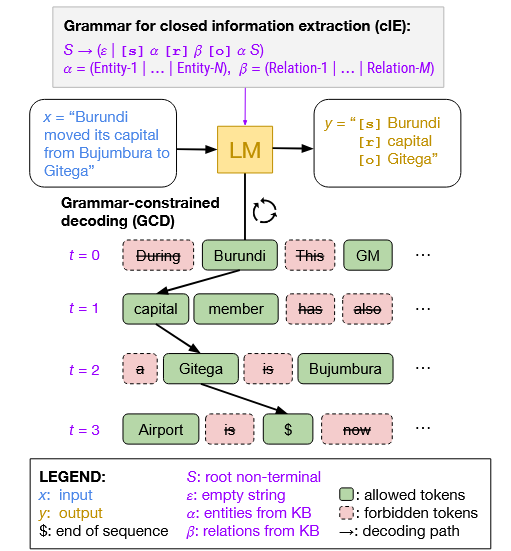
\includegraphics[width=0.45\textwidth]{Graphics/gcd.png}
\caption{Imagen extraída de \textcite{geng2023grammar}: \textit{Grammar-Constrained Decoding (GCD)} aplicado a la tarea de \textit{closed information extraction}, donde el objetivo es extraer una lista $y$ de tripletes sujeto–relación–objeto del texto de entrada $x$. Los sujetos y objetos están restringidos a ser entidades de \textit{Wikidata}, y las relaciones a ser una relación de \textit{Wikidata}. Durante la decodificación, solo se consideran continuaciones de \textit{tokens} válidas que cumplen con la gramática. Por simplicidad, se omiten los símbolos de marcador especiales \texttt{[s]}, \texttt{[r]} y \texttt{[o]} en el esquema del proceso de generación.}
\label{fig:domains}
\end{figure}

Este mecanismo es compatible con cualquier algoritmo de decodificación (como \textit{greedy decoding}, \textit{beam search}, \textit{top-$k$ sampling}, entre otros) y puede aplicarse a cualquier modelo de lenguaje autorregresivo que ofrezca acceso a su distribución de salida \textit{token} a \textit{token}. Sin embargo, es importante notar que servicios como los ofrecidos por OpenAI mediante \textit{API} no permiten acceso a dicha distribución, lo que imposibilita el uso directo de \textit{GCD} en estos contextos.

La técnica también puede combinarse eficazmente con \textit{Few-Shot Prompting}. En lugar de permitir que el modelo genere texto libre condicionado a los ejemplos del \textit{prompt}, \textit{GCD} impone una gramática que define la estructura válida de la salida esperada, restringiendo así el espacio de búsqueda y guiando al modelo hacia soluciones sintácticamente correctas. Esto permite aprovechar el conocimiento previo del modelo junto con una especificación formal del dominio de salida, lo que resulta particularmente útil en tareas estructuradas donde se requiere una alta precisión en el formato.

El enfoque de \textit{GCD} representa así una herramienta crucial para la generación segura y verificable de texto estructurado, habilitando aplicaciones en modelado de código, extracción de información, y como se explorará más adelante, en la generación de descripciones válidas en \textit{PDDL}.

\subsection{\textit{Backus-Naur Form} (\textit{BNF})}

La Notación de \textit{Backus-Naur} (\textit{Backus-Naur Form} - \textit{BNF}) surgió a finales de la década de 1950 como una herramienta formal para describir la sintaxis de lenguajes de programación. En 1959, John Backus propuso un conjunto de ``fórmulas metalingüísticas'' para definir la estructura del lenguaje \textit{ALGOL 58}, basándose en ideas de gramáticas libres de contexto \parencite{backus1959syntax}. Posteriormente, Peter Naur refinó esta notación en el informe de \textit{ALGOL 60} de 1963, denominándola ``Forma Normal de Backus'' (\textit{Backus Normal Form}) \parencite{backus1963revised}. Sin embargo, Donald Knuth sugirió renombrarla como \textit{Backus-Naur Form} para reconocer la contribución de Naur y evitar la confusión con otras formas normales existentes en teoría de lenguajes formales \parencite{knuth1964backus}.

\textit{BNF} es un metalenguaje que permite expresar gramáticas libres de contexto mediante reglas de producción. Cada regla tiene la forma:

\begin{verbatim}
<no-terminal> ::= <expresión>
\end{verbatim}

Donde \texttt{<no-terminal>} representa una categoría sintáctica y \texttt{<expresión>} define cómo se puede construir esa categoría utilizando otros símbolos terminales o no terminales. Por ejemplo, una regla podría ser:

\begin{verbatim}
<expresión> ::= <término> | <expresión> "+" <término>
\end{verbatim}

Esta notación facilita la definición precisa y estructurada de la sintaxis de lenguajes de programación, siendo fundamental en el desarrollo de compiladores y analizadores sintácticos.

\subsection{Extensión moderna: \textit{GBNF} en \texttt{llama.cpp}}

La notación \textit{Backus-Naur} (\textit{BNF}) ha sido fundamental en la definición formal de lenguajes de programación. Sin embargo, con el auge de los \textit{LLMs}, ha surgido la necesidad de formatos más expresivos y adaptados a estos nuevos contextos. En este sentido, fue introducida \textit{Georgi Gerganov's Machine Learning (GGML) Backus-Naur Form (GBNF)}, una extensión de \textit{BNF} diseñada específicamente para restringir y estructurar las salidas de los \textit{LLMs} en aplicaciones prácticas \parencite{ggml2023gbnf}.

\textit{GBNF} se implementa en el proyecto \texttt{llama.cpp}, una versión en \texttt{C++} de los modelos \textit{LLaMA} desarrollada por Gerganov. Esta notación permite definir gramáticas que los modelos deben seguir al generar texto, asegurando que las salidas cumplan con estructuras sintácticas específicas. A diferencia de \textit{BNF}, \textit{GBNF} incorpora características modernas similares a las expresiones regulares, lo que permite una mayor flexibilidad y control sobre las salidas generadas por los modelos \parencite{ggml2023gbnf}.

Aunque \textit{GBNF} no cuenta con una publicación académica formal, su documentación principal se encuentra en el repositorio oficial de \texttt{llama.cpp}, específicamente en el archivo \texttt{grammars/README.md}. Esta fuente proporciona ejemplos y directrices sobre cómo implementar y utilizar \textit{GBNF} en proyectos que requieren salidas estructuradas de modelos de lenguaje \parencite{ggml2023gbnf}.

En el contexto de esta tesis, \textit{GBNF} se utiliza como el mecanismo formal que habilita la aplicación práctica de \textit{GCD} para el modelado automático de problemas en \textit{PDDL}. Al restringir la salida de un \textit{LLM} mediante una gramática \textit{GBNF}, se garantiza que las descripciones generadas sean sintácticamente válidas conforme a la especificación del lenguaje objetivo, facilitando tanto su validación como su posterior análisis por planificadores clásicos.

\subsection{Aplicaciones Previas de \textit{GCD} en planificación automática}

\textbf{\textit{Grammar Prompting for Domain-Specific Language Generation with Large Language Models}} \parencite{wang2023grammar} propone una técnica denominada \textit{grammar prompting}, que permite a los \textit{LLMs} generar la gramática, expresada en \textit{BNF}, que seguirán sus salidas posteriores mediante \textit{GCD}. En el contexto de planificación, el modelo primero predice una gramática especializada para una tarea dada y luego genera un plan \textit{PDDL} que cumple con dicha gramática. Aunque este enfoque logra mejoras en la generación de planes sintácticamente válidos, se centra únicamente en la producción de planes, no en la generación completa de modelos de problemas de planificación.

Por otro lado, \textbf{\textit{Syntactic and Semantic Control of Large Language Models via Sequential Monte Carlo}} \parencite{loula2025syntactic} introduce un marco basado en \textit{Sequential Monte Carlo} para controlar la generación de texto por \textit{LLMs} bajo restricciones sintácticas y semánticas. Aplicado a la generación de modelos \textit{PDDL}, este enfoque utiliza una gramática \textit{STRIPS} general y se limita al dominio de \textit{Blocksworld} del \textit{benchmark Planetarium} con hasta 10 objetos, asumiendo que el estado inicial (\texttt{:init}) es proporcionado. Sus resultados experimentales brindaron indicios positivos de la utilidad de \textit{GCD} para el modelado de tareas de planificación. Sin embargo, aunque el método propuesto en el artículo permite una generación más controlada y coherente, su dependencia de información previa sobre el estado inicial restringe su capacidad para generar modelos completos a partir de descripciones en lenguaje natural. Además, no se hace una exploración a profundidad de la técnica al limitarse a un subconjunto muy reducido y solo parcialmente representativo de \textit{Planetarium}.

En contraste, esta tesis propone un enfoque que utiliza \textit{GCD} para la generación completa de modelos \textit{PDDL} (incluyendo \texttt{:init}, \texttt{:goal}, \texttt{:objects}, etc.) a partir de descripciones en lenguaje natural y del dominio \textit{PDDL} correspondiente. Más aún, se evalúa en todas las dimensiones (dominio, cantidad de objetos, nivel de abstracción, etc.) del \textit{benchmark Planetarium}. De forma adicional a la gramática general, se introducen nuevos niveles de restricción especializada que aseguran el uso exclusivo de predicados disponibles, objetos declarados y la correcta aridad y tipado de argumentos, permitiendo así una generación más precisa y aplicable a una variedad de dominios y problemas específicos.

\section{El \textit{Benchmark Planetarium}}

La evaluación moderna de modelos generados automáticamente en \textit{PDDL} requiere herramientas específicas que permitan analizar no solo la validez sintáctica del código, sino también su estructura semántica y capacidad de resolución. En esta línea, el \textit{benchmark Planetarium} \parencite{zuo2024planetarium} constituye una de las contribuciones más destacadas, al ofrecer un conjunto masivo de ejemplos texto--\textit{PDDL} junto con un protocolo de evaluación riguroso basado en estructuras de grafo intermedias. Este recurso permite evaluar la generación automática de problemas de planificación desde descripciones en lenguaje natural con criterios que trascienden la simple exactitud textual o el \textit{string matching}.

La representación central empleada por \textit{Planetarium} es el \textit{scene graph} (grafo de escena), una estructura de datos ampliamente utilizada en visión por computadora y gráficos computacionales para representar objetos, sus atributos y relaciones. Formalmente, un \textit{scene graph} es un grafo dirigido $\mathcal{G} = (\mathcal{V}, \mathcal{E})$, donde $\mathcal{V} = \mathcal{O} \cup \mathcal{P}$ incluye nodos de tipo objeto ($\mathcal{O}$) y proposición ($\mathcal{P}$), y cada arista $e \in \mathcal{E}$ tiene atributos que codifican el predicado al que pertenece, la posición del argumento en la proposición, y si la proposición corresponde al estado inicial o al estado meta. Para cada archivo de problema en \textit{PDDL}, se construyen dos grafos: uno que representa el estado inicial y otro que representa las proposiciones objetivo. Estos se combinan en un \textit{problem graph}, definido como la unión etiquetada de ambos: 

\[
\textit{ProblemGraph} = (\mathcal{O} \cup \mathcal{P}_{\textit{init}} \cup \mathcal{P}_{\textit{goal}}, \mathcal{E}_{\textit{init}} \cup \mathcal{E}_{\textit{goal}})
\]

La noción de equivalencia entre problemas se formaliza como un isomorfismo de grafos sobre los \textit{problem graphs}, es decir, una biyección entre nodos que preserve tanto la conectividad como los tipos y atributos. Esta definición permite comparar problemas generados automáticamente contra su referencia canónica sin depender del soporte textual de los archivos.

El algoritmo propuesto para verificar esta equivalencia comienza transformando cada conjunto de proposiciones en grafos de escena, completando los grafos objetivo con aristas triviales (como proposiciones que se pueden inferir verdaderas), y finalmente construyendo un \textit{problem graph} a partir de la unión. Si existe un isomorfismo entre el grafo generado y el de referencia, se considera que el problema es estructuralmente equivalente y, por tanto, correcto.

El conjunto de datos de \textit{Planetarium} incluye más de 100\,000 pares texto--\textit{PDDL}, generados proceduralmente a partir de plantillas que combinan configuraciones (subtipos de estados o subtareas específicas) de los estados iniciales y objetivos. Los dominios utilizados son \textit{Blocksworld}, \textit{Gripper} y \textit{Floor-Tile}, elegidos por su uso extensivo en la literatura y su dificultad inherente. Cada problema contiene tanto una descripción en lenguaje natural como una instancia en \textit{PDDL} construida a partir de la combinación de las plantillas predefinidas. La generación automática varía sistemáticamente la abstracción de las descripciones textuales (desde descripciones explícitas hasta resúmenes abstractos de estados) y el tamaño de los problemas medido por la cantidad total de proposiciones u objetos.

\begin{figure}[H]
\centering
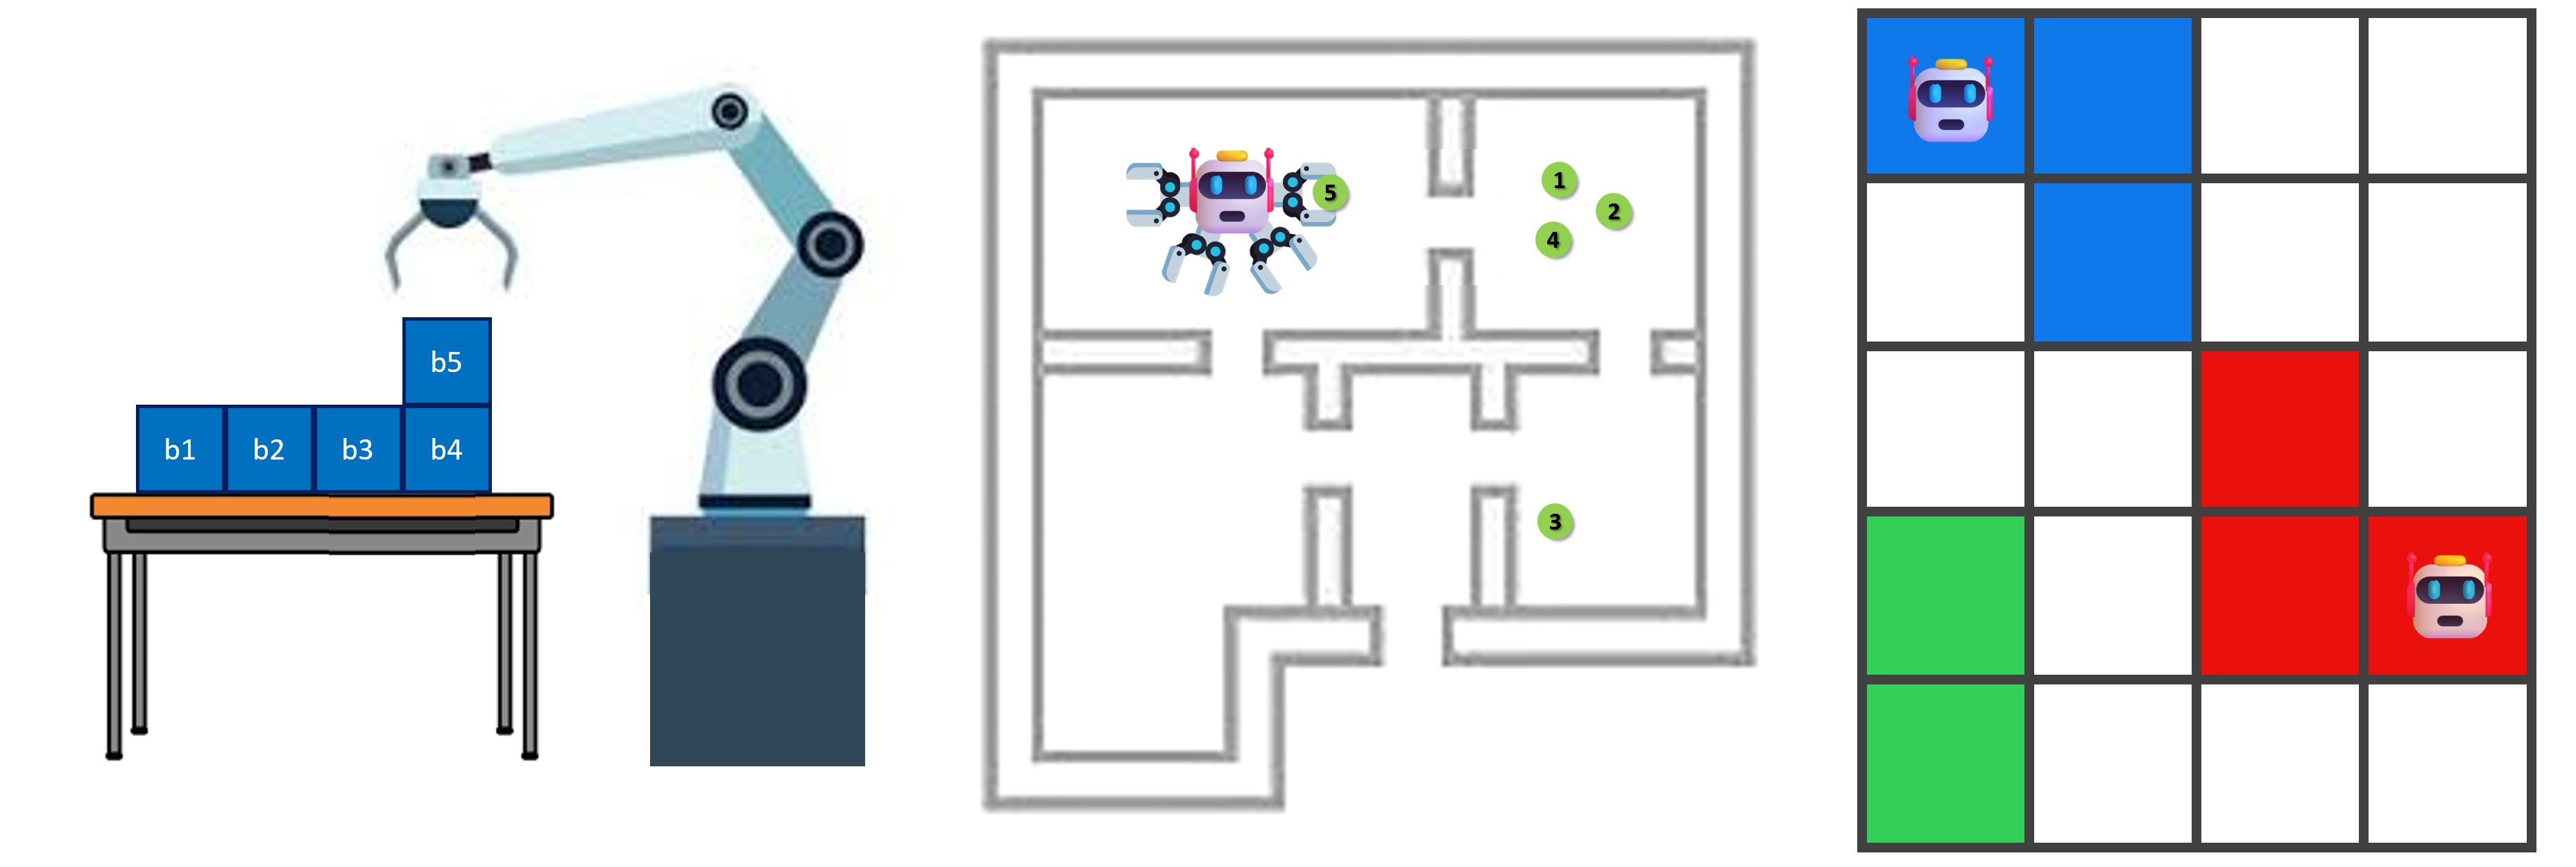
\includegraphics[width=0.8\textwidth]{Graphics/domains.png}
\caption{Dominios de problemas de planificación del \textit{benchmark Planetarium}, de izquierda a derecha: \textit{Blocksworld}, \textit{Gripper} y \textit{Floor-Tile}}
\label{fig:domains}
\end{figure}

El protocolo de evaluación del dataset considera tres métricas: el número de modelos sintácticamente válidos, el número de modelos solubles y el número de modelos correctos. Un modelo es considerado sintácticamente válido si es analizable por un \textit{parser} de \textit{PDDL}, y es posible extraer desde su salida un problema en \textit{PDDL} válido y convertirlo en un grafo estructuralmente bien formado. La solubilidad se computa determinando la existencia de un plan válido que lleva desde el estado inicial al estado objetivo, utilizando para ello planificadores específicos para los dominios \textit{Blocksworld} y \textit{Gripper}, y \textit{Fast Downward} para problemas del dominio \textit{Floor-Tile}. Finalmente, un problema se considera correcto si, siendo sintácticamente válido y soluble, es también estructuralmente equivalente al problema original según el algoritmo de isomorfismo de grafos. Para asegurar la validez de los planes generados, todos los resultados se verifican con la herramienta \textit{VAL}.

\begin{figure}[H]
\centering
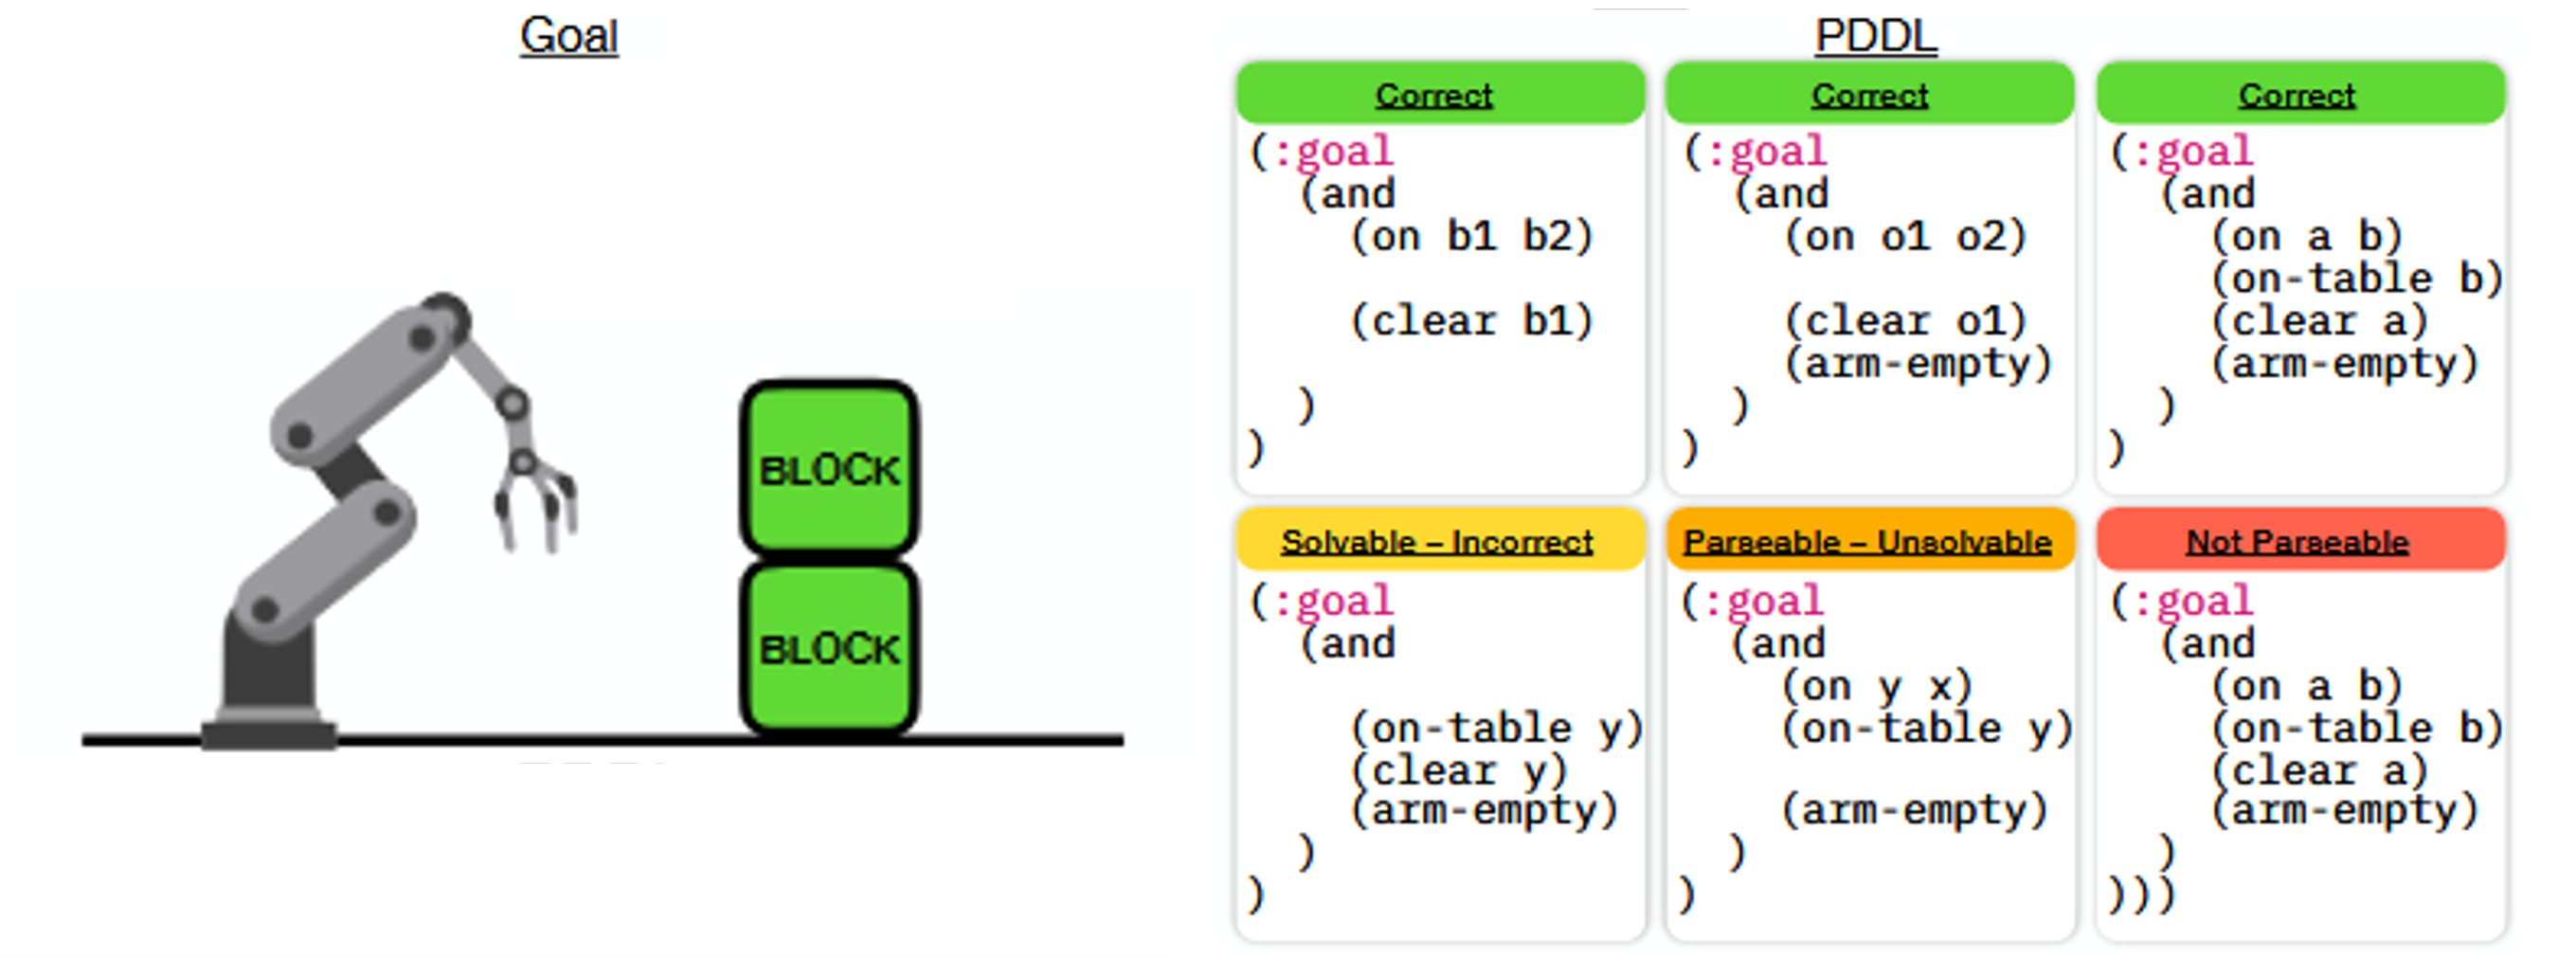
\includegraphics[width=0.9\textwidth]{Graphics/planetarium.png}
\caption{Imagen extraída del \textit{paper} de \textit{Planetarium} \parencite{zuo2024planetarium}: ejemplo de cómo un único objetivo de planificación puede corresponder a múltiples estados objetivos \textit{PDDL} correctos. Todos los objetivos \textit{PDDL} en la fila superior representan la meta mostrada correctamente. La fila inferior ilustra objetivos \textit{PDDL} con diferentes tipos de errores, mostrando instancias que son solubles (un planificador puede generar un plan, pero para un problema de planificación diferente), sintácticamente válidos (la sintaxis \textit{PDDL} es correcta pero no producirá ningún plan con un planificador) e inválidos (contiene errores de sintaxis).}
\label{fig:planetarium}
\end{figure}

Este protocolo permite una evaluación robusta de modelos basados en lenguaje natural y ofrece un \textit{baseline} reproducible para medir avances en la generación automática de modelos de planificación.

\section{Conclusiones}

Este capítulo ha presentado un recorrido exhaustivo por los fundamentos, avances y desafíos actuales en el campo de la \textit{planificación automática}, así como por las oportunidades emergentes que surgen del uso de \textit{LLMs} para la generación estructurada de modelos en \textit{PDDL}. 

En conjunto, se evidencia que, si bien los \textit{LLMs} poseen un enorme potencial para tareas de planificación estructurada, su aplicación directa a la generación de modelos \textit{PDDL} enfrenta barreras significativas de robustez y validación. Las técnicas revisadas —aprendizaje experiencial, decodificación gramatical, evaluación estructural con \textit{Planetarium}— ofrecen elementos clave para superar estas barreras. Sobre esta base se plantea en esta tesis el diseño de un agente modelador que:
\begin{itemize}
    \item Divide el proceso de modelado en fases de razonamiento estructurado, extracción de objetos y generación de \textit{PDDL};
    \item Aprende de sus errores mediante ciclos de experiencia y reflexión;
    \item Está asistido por restricciones gramaticales explícitas mediante \textit{GCD} y \textit{GBNF};
    \item Es evaluado rigurosamente con el protocolo estructural de \textit{Planetarium}.
\end{itemize}

Este enfoque integral busca cerrar la brecha entre el poder expresivo de los \textit{LLMs} y la precisión requerida por los sistemas simbólicos de planificación, contribuyendo así a un nuevo paradigma de generación automática de modelos válidos, verificables y reutilizables en el contexto de la \textit{planificación automática}.
